\documentclass[aspectratio=169]{beamer}
\usetheme{boxes}
\usepackage{essay-def}
\usepackage{bm}
\usepackage{booktabs}
\usepackage{amsfonts}
\usepackage{amssymb}
\usepackage{amsmath}
\usepackage{amsthm}
\usepackage{comment}
\usepackage{enumitem}
\usepackage{geometry}
\usepackage{algorithmic}
\usepackage{algpseudocode}
\usepackage{algorithmicx}
\usepackage{graphicx}
\usepackage{subcaption}
\usepackage{tikz}
\usepackage{physics}
\usepackage{xcolor}
\usepackage{enumitem}
\setitemize{label=$\circ$}
\setbeamertemplate{itemize subitem}{\textbullet}
\usepackage[version=4]{mhchem}
\geometry{left=1cm,right=1cm}
\title[ML4DFT]{Machine Learning-Inspired Advancements in Density Functional Theory}
\author[J. Zhao]{Jiaxi Zhao (NUS) \\ joint with Tianbo Li, Zekun Shi, and Min Lin
@ SAIL\\
Giovanni Vignale and Qianxiao Li @ NUS}
\date[\today]{\today\\
Job talk @ Bytedance}

% TODO: add reference to each slide, better use a concise notion
\begin{document}
% \par \setlength{\parindent}{2em}

\begin{frame}
\titlepage
\end{frame}


\begin{frame}{Research}
	\begin{itemize}
		\item Applied mathematics Ph.D. @ National University of Singapore
		developing data-driven hybrid simulation method for PDE problems
		\begin{itemize}
			\item {\scriptsize \color{red} Mitigating distribution shift in machine learning-augmented hybrid simulation (SISC 2025)}
			\item {\scriptsize \color{red} Generative subgrid-scale modeling (MLMP ICLR 2025)}
			\item {\scriptsize Numerical analysis on neural network projected schemes for approximating one dimensional Wasserstein gradient flows (JCP 2025)}
			\item {\scriptsize Variational conditional normalizing flows for computing second-order mean field control problems}
			\item {\scriptsize Numerical analysis for data-driven SGS modeling}
		\end{itemize}
		\item Research intern @ Sea AI Lab improving the jax-based
		solid-state DFT solver \textit{Jrystal} (core developer) using machine-learning toolbox
		\begin{itemize}
			\item {\scriptsize Amortized Eigendecomposition for Neural Networks (NeurIPS 2024)}
			\item {\scriptsize \color{red} Normalizing Flow Distorted Planewaves}
			\item {\scriptsize \color{red} Adaptive Gaussian basis for quantum chemistry calculation}
			\item {\scriptsize Benchmarking occupation parametrizations in direct optimization approach for solid-state density functional theory}
		\end{itemize}
	\end{itemize}
\end{frame}


% \begin{frame}{Outline}
% 	\tableofcontents
% \end{frame}


\begin{frame}{Three fundamental difficulties of DFT}
	\begin{equation*}
		\begin{aligned}
			\delta E[\phi_k^*(x_k)] & \ = \delta E(\phi_1, \phi_2, \cdots, \phi_N)
			- \delta\left[\sum_{i=1}^N \sum_{j=1}^N
			\lambda_{ij} \left( \left\langle\phi_i, \phi_j\right\rangle - \delta_{ij}
			\right)\right]		\\
			\wht \opF(\text{k})\phi_k(\mathbf{r}_k) & \equiv \left[ \hat{h}
			(\text{k}) + \hat{J}(\text{k}) - \hat{K}(\text{k}) \right]
			\phi_k(\mathbf{r}_k) = \epsilon_k \phi_k(\mathbf{r}_k),	\\
			\wht \opJ(\text{k}) & \equiv \sum_{j=1}^N \int \mathrm{d}\mathbf{r}_j
			\frac{\phi_j^*(\mathbf{r}_j) \phi_j(\mathbf{r}_j)}{|\mathbf{r}_k-
			\mathbf{r}_j|}= \sum_{j=1}^N \int \mathrm{d}\mathbf{r}_j \frac{\rho(
			\mathbf{r}_j)}{|\mathbf{r}_k-\mathbf{r}_j|},\\
			\wht \opK(\text{k})\phi_{k}(\mathbf{r}_k) & \equiv  \sum_{j=1}^N
			\phi_{j}(\mathbf{r}_k) \int \text{d}\mathbf{r}_j \frac{\phi_j^*
			(\mathbf{r}_j) \phi_k(\mathbf{r}_j)}{|\mathbf{r}_k-\mathbf{r}_j|}.\\
		\end{aligned}
	\end{equation*}
	\begin{itemize}
		\item Complexity of the basis set $\Longrightarrow$ Adaptive Gaussian basis set
		\item High plane-waves cutoff for crystal system $\Longrightarrow$ Normalizing Flow Distorted Planewaves
		\item XC functional for materials $\Longrightarrow$ MLXC under PAW formulation
	\end{itemize}
\end{frame}


\begin{comment}
% for long talk
\begin{frame}{Many-body Schr\"odinger equation}
	After Born–Oppenheimer approximation, the many-body Schr\"odinger equation
	is given by:
	\begin{equation*}
		\begin{aligned}
			\hat{\opH^e} & \Psi(\mfr_1, \mfr_2, ..., \mfr_N) = E
			\Psi(\mfr_1, \mfr_2, ..., \mfr_N),		\\
			\hat{\opH^e} & = -\half \Delta_{\mfr} - \sum_{i=1}^N\sum_{j=1}^{n_A} \frac{Z_j}
			{\norml \mfr_i - \mfR_j \normr_2} + \frac{1}{2} \sum_{i \neq j}^N
			\frac{1}{r_{ij}}		\\
			& = \sum_{i=1}^N \wht{\operatorname{h}}(\text{i}) + \frac{1}{2} \sum_{i \neq j}^N
			\frac{1}{r_{ij}}
		\end{aligned}
	\end{equation*}
	Solving this equation, we can obtain the ground state energy, potential
	energy surface (for geometry optimization and transition states search),
	band structure for the solid state system, and etc.
\end{frame}


% for long talk
\begin{frame}{Mean-field approximation: Slater determinant}
	Pauli exclusion principle requires following antisymmetric constraint on the
	many-body wave function:
	\begin{equation*}
		\Psi(..., \mfr_j, ..., \mfr_i, ...) = 
		- \Psi(..., \mfr_i, ..., \mfr_j, ...)
	\end{equation*}

	The many-body wave function of the Hartree-Fock theory is given by a single
	Slater determinant:
	\begin{equation*}
		\Psi_{\text{HF}}(\mfr_1, ..., \mfr_N) = \frac{1}{\sqrt{N!}} 
		\begin{vmatrix}
			\phi_1(\mfr_1) & \phi_1(\mfr_2) & \cdots & \phi_1(\mfr_N) \\
			\phi_2(\mfr_1) & \phi_2(\mfr_2) & \cdots & \phi_2(\mfr_N) \\
			\vdots & \vdots & \ddots & \vdots \\
			\phi_N(\mfr_1) & \phi_N(\mfr_2) & \cdots & \phi_N(\mfr_N)
		\end{vmatrix}
	\end{equation*}
\end{frame}

% for long talk
\begin{frame}{Total energy}
	\begin{equation*}
		\begin{aligned} & E[\Psi^{HF}] = 
			\left\langle\Psi^{HF}|\hat{\opH^e}|\Psi^{HF}
			\right\rangle =  \sum_{i=1}^N \int\text{d}\mathbf{r}_i
		  \phi_i^*(\mathbf{r}_i)
			\wht{\operatorname{h}}(\text{i}) \phi_i(\mathbf{r}_i) \\ 
			&+ \frac{1}{2N(N - 1)} \sum_{i \neq j}^N \sum_{k \neq l}^N \iint
			\mathrm{d}\mathbf{r}_i
			\text{d}\mathbf{r}_j \phi_k^*(\mathbf{r}_i)\phi_l^*(\mathbf{r}_j)
			\frac{1}{|\mathbf{r}_i-\mathbf{r}_j|}\phi_k(\mathbf{r}_i)
			\phi_l(\mathbf{r}_j) \\ 
			&- \frac{1}{2N(N - 1)} \sum_{i \neq j}^N \sum_{k \neq l}^N \iint
			\text{d}\mathbf{r}_i
			\text{d}\mathbf{r}_j\phi_k^*(\mathbf{r}_i)\phi_l^*(\mathbf{r}_j)
			\frac{1}{|\mathbf{r}_i-\mathbf{r}_j|}\phi_k(\mathbf{r}_j)
			\phi_l(\mathbf{r}_i)  \\
			& = E(\phi_1, \phi_2, \cdots, \phi_N).
		\end{aligned}
	\end{equation*}
	Minimizing the total energy will give the ground state configuration which is
	consistent with the self-consistent field approach. The double-electron
	integrations $O(N^4)$ are the dominant part of computational cost.
\end{frame}

\begin{frame}{Mathematical formulation}
	Variational formulation of the Hartree-Fock theory:
	\begin{equation*}
		\begin{aligned}
			& E(\phi_1, \phi_2, \cdots, \phi_N) = 
	\sum_{i=1}^N \int\text{d}\mathbf{r}_i
		  \phi_i^*(\mathbf{r}_i) (-\frac{1}{2}\Delta - \sum_{\text{atom } a}
			\frac{Z_a}{|\mathbf{r}_i - \mathbf{A}_a|})(\mathbf{r}_i))
			 \phi_i(\mathbf{r}_i) \\ 
			&+ \frac{1}{2N(N - 1)} \sum_{i \neq j}^N \sum_{k \neq l}^N \iint
			\mathrm{d}\mathbf{r}_i
			\frac{1}{|\mathbf{r}_i-\mathbf{r}_j|}
			\left(\underbrace{\phi_l(\mathbf{r}_j)\phi_l^*(\mathbf{r}_j)}_{\rho_l(\mathbf{r}_j)}
			\text{d}\mathbf{r}_j \overbrace{\phi_k^*(\mathbf{r}_i)\phi_k(\mathbf{r}_i)
			}^{\rho_k(\mathbf{r}_i)} - \underbrace{\phi_k^*(\mathbf{r}_i)\phi_l^*(\mathbf{r}_j)
			\phi_k(\mathbf{r}_j)\phi_l(\mathbf{r}_i)}_{\text{Exchange term}}\right)  \\
      & \int\text{d}\mathbf{r}
		  \phi_i^*(\mathbf{r}) \phi_j(\mathbf{r}) = \delta_{ij}.
		\end{aligned}
	\end{equation*}
	\begin{itemize}
		\item Mean-field approximation of the quantum many-body Schr\"odinger equation.
		\item Direct optimization of the total energy; self-consistent field (SCF) method.
		\item Discretization of the wave function: $\phi_j = \sum_{i\in I} c_{ji}\varphi_i$.
	\end{itemize}
\end{frame}
\end{comment}


\section{Adaptiv Gaussian basis for quantum chemistry calculation}
\begin{frame}
    \centering
    \Large
    \textcolor{blue}{\insertsection}\\
		\vspace{1cm}
		\normalsize
		Jiaxi Zhao, Giovanni Vignale, and Min Lin
\end{frame}


\begin{frame}{Basis sets are complicated}
	\begin{itemize}
		\item Slater basis functions (STO):
		\begin{equation*}
			\varphi^{\opS} \equiv \text{poly}(x, y, z)
			e^{-\alpha \norml \mfr - \mfA \normr_2}
		\end{equation*}
		\item Gaussian basis functions (GTO):
		\begin{equation*}
			\varphi^{\opG} \equiv \text{poly}(x, y, z)
			e^{-\alpha \norml \mfr - \mfA \normr_2^2}
		\end{equation*}
		\item Numerical atomic orbitals:
		\begin{equation*}
			\varphi^{\text{NAO}} \equiv \sum_{L}^{L_A}
			Y_L(\widehat{\mathbf{r} - \mathbf{A}})
			f_L(\norml \mathbf{r} - \mathbf{A} \normr_2^2)
		\end{equation*}
	\end{itemize}
\end{frame}

% for long talk
\begin{frame}{Basis sets integrals are computationally expensive}
	\begin{equation*}
		\iint e^{-\alpha \norml \mfr_1 - \mfA \normr_2^2 -\beta \norml \mfr_2 - \mfB \normr_2^2
		-\gamma \norml \mfr_1 - \mfC \normr_2^2 -\delta \norml \mfr_2 - \mfD \normr_2^2}
		\frac{\text{poly}(\mfr_1, \mfr_2)}{r_{12}}d\mfr_1d\mfr_2
	\end{equation*}
	\begin{itemize}
		\item Boys' rule
		\item Classical recursive-based method: MD, HPG, Rys
		\item Higher angular-momentum integrals become very expensive to calculate
		\item {\color{red}\textbf{Basis set optimization}} is also a hot topic for research
	\end{itemize}
\end{frame}

\begin{frame}{Adaptive Gaussian basis}
	% Classically, basis set of increasing complexity is used to 
	% \begin{itemize}
	% 	\item 1. STO-n 
	% 	\item 2. 6-311G*
	% 	\item 3. cc-pVDZ
	% \end{itemize}

	Adaptive Gaussian basis (Kerbl, Bernhard, et al 2023) with optimizable mean and covariance:
	\begin{equation*}
		\phi_i = \sum_{j\in I} c_{ij}\mcN(\mfr; \mu_j, \Sigma_j)
	\end{equation*}
	In general, all the optimizable parameters are $\mu \in \mbR^{|I|\times 3},
	\Sigma \in \lp \mbS_+^3 \rp^{|I|}, C \in \mbC^{|I|\times N}$. $|I|$ is the
	size of the basis set, $N$ is the number of electrons

	\begin{itemize}
		\item Polynomial to more flexible covariance structure
		\item Analytic Gaussian integral
	\end{itemize}
\end{frame}

\begin{frame}{Orthonormality and overlap matrix}
	\begin{itemize}
		\item The orthonormality of the orbitals in SCF is guaranteed by the eigensolver
		\item In total energy minimization, we have to handle this explicitly
	As the orbitals are supposed to be orthonormal, it can be written as
	\begin{equation*}
		\opC^{\dagger} \opS \opC = \opI
	\end{equation*}
	where $\opS$ is the overlap matrix defined as:
	\begin{equation*}
		\operatorname{S}_{ij} = \la \mcN\lp \mfr; \mathbf{\mu_i},
    \Sigma_i \rp \rv \left. \mcN\lp \mfr;
    \mathbf{\mu_j}, \Sigma_j \rp \ra
	\end{equation*}
	The orthonormality is enforced by QR decomposition modified by the
	Cholesky factorization of $\opS$
	\end{itemize}
\end{frame}

\begin{frame}{Coulomb and external energy}
	\begin{itemize}
		\item No analytic formula for electron repulsion integral (ERI)
		\begin{equation*}
			\la \mcN\lp \mfr_1 | \mathbf{\mu_1}, \Sigma_1 \rp \rv \frac{1}{
					\lv \mfr_1 - \mfr_2 \rv}\lv \mcN\lp \mfr_2 | \mathbf{\mu_2}, \Sigma_2
					\rp \ra
		\end{equation*}
		\item Approximate the Coulomb kernel by a series of
		Gaussian modes:
		\begin{equation*}
			\frac{1}{r} = \sum_i c_i e^{-\alpha_i r^2}
		\end{equation*}
		\item Minimizing the following
		\begin{equation*}
			\begin{aligned}
				\min_{c_i, \alpha_i} \int_{B_M} \lp \frac{1}{|\mfr|} - \sum_i c_i
				e^{-\alpha_i |\mfr|^2} \rp^2 d\mfr = 4\pi\int_0^M \lp 1 - \sum_i c_i
				re^{-\alpha_i r^2} \rp^2 dr
			\end{aligned}
		\end{equation*}
	\end{itemize}
\end{frame}

% for long talk
% \begin{frame}{Analysis of the nonlinear optimization problem}
% 	\begin{equation*}
% 		\begin{aligned}
% 			& \ \int_0^M \lp 1 - \sum_i c_i re^{-\alpha_i r^2} \rp^2 dr 
% 			\overset{u = kr}{=} & \ \frac{1}{k}\int_0^{kM} \lp 1 - \sum_i \frac{c_i}{k} u 
% 			e^{-\frac{\alpha_i}{k^2} u^2} \rp^2 du.
% 		\end{aligned}
% 	\end{equation*}
% 	The optimal solution for different $M$ can be obtained by rescaling the optimal
% 	coefficient and variance of the Gaussian modes.

% 	However, optimizing such problem to a relatively low threshold, e.g. $10^{-5}$
% 	is quite difficult.
% 	\begin{figure}[h]
% 		\centering
% 		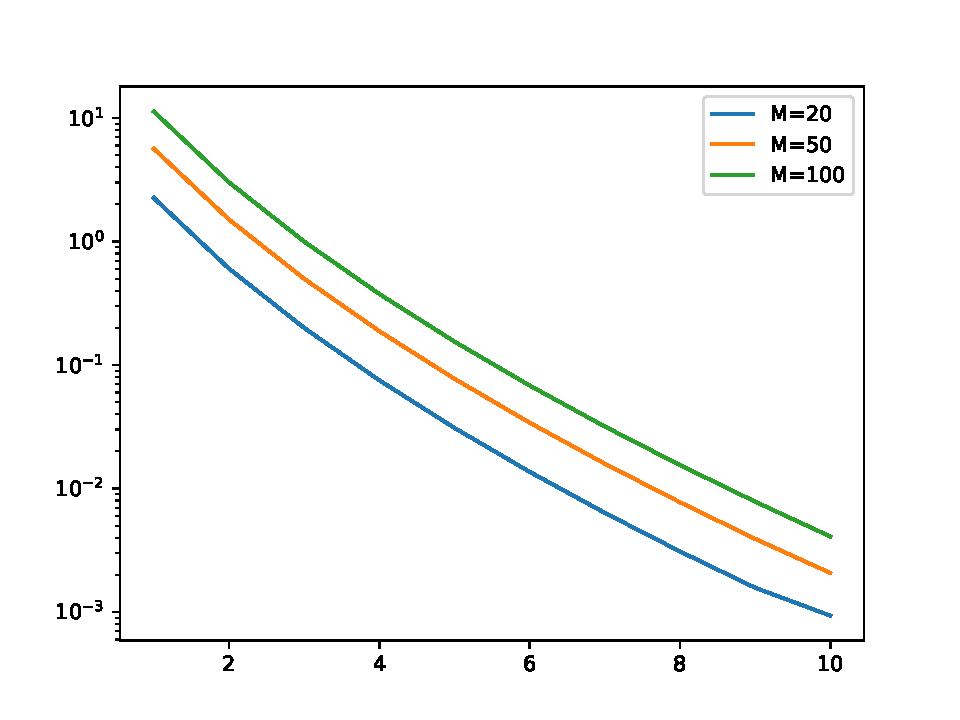
\includegraphics[width=0.5\linewidth]{fig/convergence.pdf}
% 	\end{figure}
% \end{frame}


\begin{frame}{More on double electron integrals}
	\tinysize
	\begin{equation*}
		\begin{aligned}
			& \ \la \mcN\lp \mfr_1 | \mathbf{\mu_1}, \Sigma_1 \rp \rv \frac{1}{
				\lv \mfr_1 - \mfr_2 \rv}\lv \mcN\lp \mfr_2 | \mathbf{\mu_2}, \Sigma_2
				\rp \ra     \\
			= & \ \int\int d\mfr_1d\mfr_2 \frac{1}{\sqrt{(2\pi)^6\det(\Sigma_1)
			\det(\Sigma_2)}} \sum_i c_i  \exp\lb -\half\lp (\mfr_1 - \mu_1)^T
			\Sigma_1^{-1}(\mfr_1 - \mu_1) \right.\right.		\\
				& \ \left.\left. + (\mfr_2 - \mu_2)^T\Sigma_2^{-1}(\mfr_2 - \mu_2)\rp
				- (\mfr_1 - \mfr_2)^T \alpha_i \operatorname{I} (\mfr_1 - \mfr_2) \rb
			\\
			= & \ \int\int d\mfr \frac{\sum_i c_i s(i)\exp\lb -\half(\mfr - \mu(i))^T \begin{pmatrix}
				\Sigma_1^{-1} + 2\alpha_i \operatorname{I} & -2\alpha_i \operatorname{I}
				\\
				-2\alpha_i \operatorname{I} & \Sigma_2^{-1} + 2\alpha_i \operatorname{I}
				\end{pmatrix} (\mfr - \mu(i)) \rb}{\sqrt{(2\pi)^6\det(\Sigma_1)
			\det(\Sigma_2)}}
		\end{aligned}
	\end{equation*}
	\begin{itemize}
		\item Solving a linear system of size $3\times 3$, MVP of size $3\times 3$, calculating
		the determinant of a $3\times 3$ matrix
	\end{itemize}
\end{frame}


\begin{frame}{Parameterization of Gaussian basis}
	We parameterize the Gaussian basis as
	\begin{equation*}
		\Sigma_1 = \opU_1 \opD_1 \opU_1^T, \quad \Sigma_2 = \opU_2 \opD_2 \opU_2^T
	\end{equation*}
	where $\opU_i$ is obtained from the QR decomposition and the positivity of
	the diagonal element of $\opD_i$ is enforced by the softplus function

	This is proved to be more robust than parametrization by Cholesky
	factorization
\end{frame}


\begin{frame}{The core contribution of this work}
	\begin{itemize}
		\item A self-contained integral library for the Hartree-Fock calculation
		using the Gaussian basis functions with more flexible covariance
		\item A complete unit test to verify the correctness of the integral
		\item Efficient Fock build algorithm: single ERI
		evaFLOPs count around $60 \times 10 = 600$, \textbf{regardless of the orbital type!}
		\item Classical Fock build algorithm: (ss|ss), (ps|ps), (pp|pp) requires 33, 58, 1326 FLOPs
		for a single evaluation (Barca et al 2020, 2021)
	\end{itemize}
\end{frame}


\begin{frame}{Numerical experiments}
	\begin{table}[tb]
		\centering
		\Large
		\resizebox{0.95\columnwidth}{!}{
		\begin{tabular}{P{4cm} P{2cm} P{2cm} P{2cm} P{2cm} P{2cm} P{2cm} P{2cm}}
		\toprule [1.5pt]
		\parbox{4cm}{  } &   \parbox{2cm}{ \centering e\_kin + e\_ext} &
		\parbox{2cm}{\centering  e\_kin}
		& \parbox{2cm}{\centering  e\_ext} & 
		\parbox{2cm}{ \centering e\_nuc } & \parbox{2cm}{ \centering 
		e\_coul + e\_exc} & \parbox{2cm}{ \centering 
		e\_coul} & \parbox{2cm}{ \centering e\_exc} & \parbox{2cm}
		{\centering  e\_tot}   \\ \midrule[1.5pt]
		
		\parbox{4cm}{OUR ($\ce{H2}$), 10} & -2.5062 & 1.1254 & -3.6316 & 0.7138 & 0.6591 &
		1.3182 & -0.6591 & \textbf{-1.1334} \\ \midrule[0.5pt]
	
		% \parbox{3cm}{$n_g= 10, \epsilon=10^{-3}$} & -2.4905 & 1.1070 & -3.5975
		% & 0.7138 & 0.6549 & 1.3097 & -0.6549 & -1.1219 \\ \midrule[0.5pt]
	
		% \parbox{3cm}{$n_g = 20, \epsilon=10^{-3}$} & -2.4897 & 1.1069 & -3.5966
		% & 0.7138 & 0.6547 & 1.3094 & -0.6547 & -1.1213 \\ \midrule[0.5pt]
	
		% \parbox{3cm}{$n_g = 20, \epsilon=10^{-4}$} & -2.4917 & 1.1095 & -3.6012
		% & 0.7138 & 0.6550 & 1.3100 & -0.6550 & -1.1229 \\ \midrule[0.5pt]
	
		% \parbox{3cm}{$n_g = 10, \epsilon=10^{-4}$} & -2.4909 & 1.1078 & -3.5987
		% & 0.7138 & 0.6550 & 1.3100 & -0.6550 & -1.1221 \\ \midrule[0.5pt]
	
		\parbox{4cm}{HF (STO-3G, 2)} 
		& -2.5049 &  * & * & 0.7138 & 0.6745 & * & * & -1.1167
		\\ \midrule[0.5pt]
	
		\parbox{4cm}{HF (6-31G, 4)} 
		& -2.4902 &  * & * & 0.7138 & 0.6497 & * & * & -1.1267
		\\ \midrule[0.5pt]
	
		\parbox{4cm}{HF (6-311G, 6)} 
		& -2.4924 &  * & * & 0.7138 & 0.6507 & * & * & \textbf{-1.1280}
		\\ \midrule[0.5pt]
	
		% \parbox{3cm}{d4ft (6-31g, lda)} 
		% & -2.482366 & * & * & 0.713754 & * & 1.280327 & -0.552556 & -1.038646
		% \\ \midrule[0.5pt]
	
		% \parbox{3cm}{pyscf} 
		% & -2.480171 & * & * & 0.713754 & * & 1.275792 & -0.554381 & -1.047201
		% \\ \midrule[0.5pt] \midrule[0.5pt]
	
		% \parbox{3cm}{OUR (\ce{CH4})} & -78.6437 & 37.8278 & -116.4715 & 13.4477
		% & 25.8757 & 32.3750 & -6.4993 & -39.3203 \\ \midrule[0.5pt]
	
		% \parbox{3cm}{$n_g = 10, \epsilon=10^{-3}$} & -78.3927 & 39.6854 &
		% -118.0781 & 13.4477 & 25.6199 & 32.2481 &
		% -6.6282 & -39.3251 \\ \midrule[0.5pt]
	
		% \parbox{3cm}{$n_g = 20, \epsilon=10^{-3}$} & -79.3790 & 39.9992 &
		% -119.3782 & 13.4477 & 26.01440 & 32.5979 &
		% -6.5835 & -39.9169 \\ \midrule[0.5pt]
	
		% \parbox{3cm}{$n_g = 20, \epsilon=10^{-4}$} & -79.2670 & 39.8448 &
		% -119.1118 & 13.4477 & 25.9379& 32.5050 &
		% -6.5671 & -39.8813 \\ \midrule[0.5pt]
	
		% \parbox{3cm}{$n_g = 10, \epsilon=10^{-4}$} & -77.5650 & 39.5177 &
		% -117.0827 & 13.4477 & 24.9640 & 31.5523 &
		% -6.5883 & -39.1532 \\ \midrule[0.5pt]
	
		\parbox{4cm}{OUR ($\ce{CH4}$), 22} & -79.6713 & 40.0987 & -119.7700 & 13.4477
		& 26.1010 & 32.6936 & -6.5926 & \textbf{-40.1225} \\ \midrule[0.5pt]
	
		\parbox{4cm}{HF (STO-3G, 9)} 
		& -79.3617 &  * & * & 13.4477 & 26.1872 & * & * & -39.7267
		\\ \midrule[0.5pt]
	
		\parbox{4cm}{HF (6-31G, 17)} 
		& -79.6901 &  * & * & 13.4477 & 26.0619 & * & * & \textbf{-40.1804}
		\\ \midrule[0.5pt]
	
		\parbox{4cm}{HF (6-311G, 25)} 
		& -79.6872 &  * & * & 13.4477 & 26.0515 & * & * & -40.1880
		\\ \midrule[0.5pt]
	
		% \parbox{3cm}{d4ft} 
		% & -79.503407 & * & * & 13.349528 & * & 32.452280 & -5.856054 & -39.467655
		% \\ \midrule[0.5pt]
	
		% \parbox{3cm}{pyscf} 
		% & -79.472583 & * & * & 13.349528 & * & 32.586078 & -5.843392 & -39.290969
		% \\ \midrule[0.5pt] \midrule[0.5pt]
	
		% \parbox{3cm}{OUR (\ce{H2O})} & -120.2329 & 68.1350 & -188.3679 & 9.1895 &
		% 37.4786 & 46.2207 & -8.7421 & -73.5648 \\ \midrule[0.5pt]
	
		% \parbox{3cm}{$n_g = 10, \epsilon=10^{-3}$} & -120.9352 & 74.8185 &
		% -195.7537 & 9.1895 & 37.0497 & 46.0144 &
		% -8.9647 & -74.6960 \\ \midrule[0.5pt]
	
		% \parbox{3cm}{$n_g = 20, \epsilon=10^{-3}$} & -122.6473 & 75.5681 &
		% -198.2154 & 9.1895 & 37.7575 & 46.6995 &
		% -8.9420 & -75.7003 \\ \midrule[0.5pt]
	
		% \parbox{3cm}{$n_g = 20, \epsilon=10^{-4}$} & -122.7171 & 75.8241 &
		% -198.5412 & 9.1895 & 37.8074 & 46.7600 &
		% -8.9526 & -75.7202 \\ \midrule[0.5pt]
	
		% \parbox{3cm}{$n_g = 10, \epsilon=10^{-4}$} & -119.5637 & 74.4819 &
		% -194.0456 & 9.1895 & 36.1289 & 45.0722 &
		% -8.9433 & -74.2454 \\ \midrule[0.5pt]
	
		\parbox{4cm}{OUR ($\ce{H2O}$), 22} & -122.9802 & 75.9462 &
		-199.0371 & 9.1895 & 37.8786 & 46.8579 &
		-8.9601 & \textbf{-76.0036} \\ \midrule[0.5pt]
	
		\parbox{4cm}{HF (STO-3G, 7)} 
		& -122.3614 &  * & * & 9.1895 & 38.2089 & * & * & -74.9630
		\\ \midrule[0.5pt]
	
		\parbox{4cm}{HF (6-31G, 13)} 
		& -122.9701 &  * & * & 9.1895 & 37.7966 & * & * & -75.9839
		\\ \midrule[0.5pt]
	
		\parbox{4cm}{HF (6-311G, 19)} 
		& -123.0146 &  * & * & 9.1895 & 37.8157 & * & * & \textbf{-76.0094}
		\\ \midrule[0.5pt]
	
		% \parbox{3cm}{d4ft} 
		% & -122.983359 & * & * & * & 9.189533 & 46.449287 & -8.117571 & -75.462110
		% \\ \midrule[0.5pt]
	
		% \parbox{3cm}{pyscf} 
		% & -122.839414 & * & * & * & 9.189534 & 46.589372 & -8.093291 & -75.153800
		% \\ \midrule[0.5pt]
	
		\\\bottomrule[1.5pt]
		\end{tabular}
		}
	\end{table}
\end{frame}


% \begin{frame}{Next step}
% 	\begin{itemize}
% 		\item 1. Compare the scalability of the double-electron integral
% 		calculation over the number of basis functions with the SOTA method, e.g.
% 		MD, HGP(OS), Rys.
% 		\item 2. Conduct numerical experiments to check if the adaptive
% 		Gaussian basis can achieve the same accuracy with a smaller number of
% 		basis.
% 		\item 3. Implement post HF method, e.g. CCSD, CCSD(T).
% 	\end{itemize}
% \end{frame}


\section{Normalizing Flow Distorted Planewaves}
\begin{frame}
	\centering
	\Large
	\textcolor{blue}{\insertsection}\\
	\vspace{1cm}
	\normalsize
	Zekun Shi, Jiaxi Zhao, and Giovanni Vignale
\end{frame}


\begin{frame}{A primer on plane-wave based solid-state DFT}
	\begin{itemize}
		\item Bloch's theorem: $\phi_j(\mathbf{r}) = e^{i\mathbf{k_j} \cdot \mathbf{r}}
		u_j(\mathbf{r})$, $u_j(\mathbf{r})$ periodic in the unit cell
		\item Basis functions: plane-waves $e^{i\mathbf{k} \cdot \mathbf{r}}, \mathbf{k}$
		lattice vector
		\item Double electron integral $\Longrightarrow$ Poisson equation (solved by FFT):
		\begin{equation*}
			\begin{aligned}
				E_{\text{Coulomb}} &= \frac{1}{2} \int_{\Omega}d\mathbf{r}\int_{\mathbb{R}^3}d\mathbf{r}' 
				\frac{\rho(\mathbf{r}) \rho(\mathbf{r'})}{\abs{\mathbf{r} - \mathbf{r'}}}d\mathbf{r} d\mathbf{r'},	\\
				E_{\text{Coulomb}} &= \frac{1}{2} \int_{\Omega}d\mathbf{r}\rho(\mathbf{r})V_{\text{H}}(\mathbf{r})d\mathbf{r},	\quad
				\nabla^2 V_{\text{H}} = -4\pi \rho(\mathbf{r})\\
			\end{aligned}
		\end{equation*}
		\item Ewald summation for nucleus repulsion energy
		\item Systematical approach to obtain more accurate DFT calculation -- increase
		the plane-wave energy cutoff
	\end{itemize}
	
	% \JX{We need to survey the literature for some multiscale basis such as
	% the wavelet basis.}
\end{frame}


\begin{frame}{Literature}
	\begin{itemize}
		\item Orbital peaks around atomx $\Longrightarrow$ High planewaves cutoff
		\item Use fixed analytic transformation mapping depending on the position of the
		atom: Gygi (1993), Zumbach et al. (1996)
		\begin{figure}[h]
			\centering
			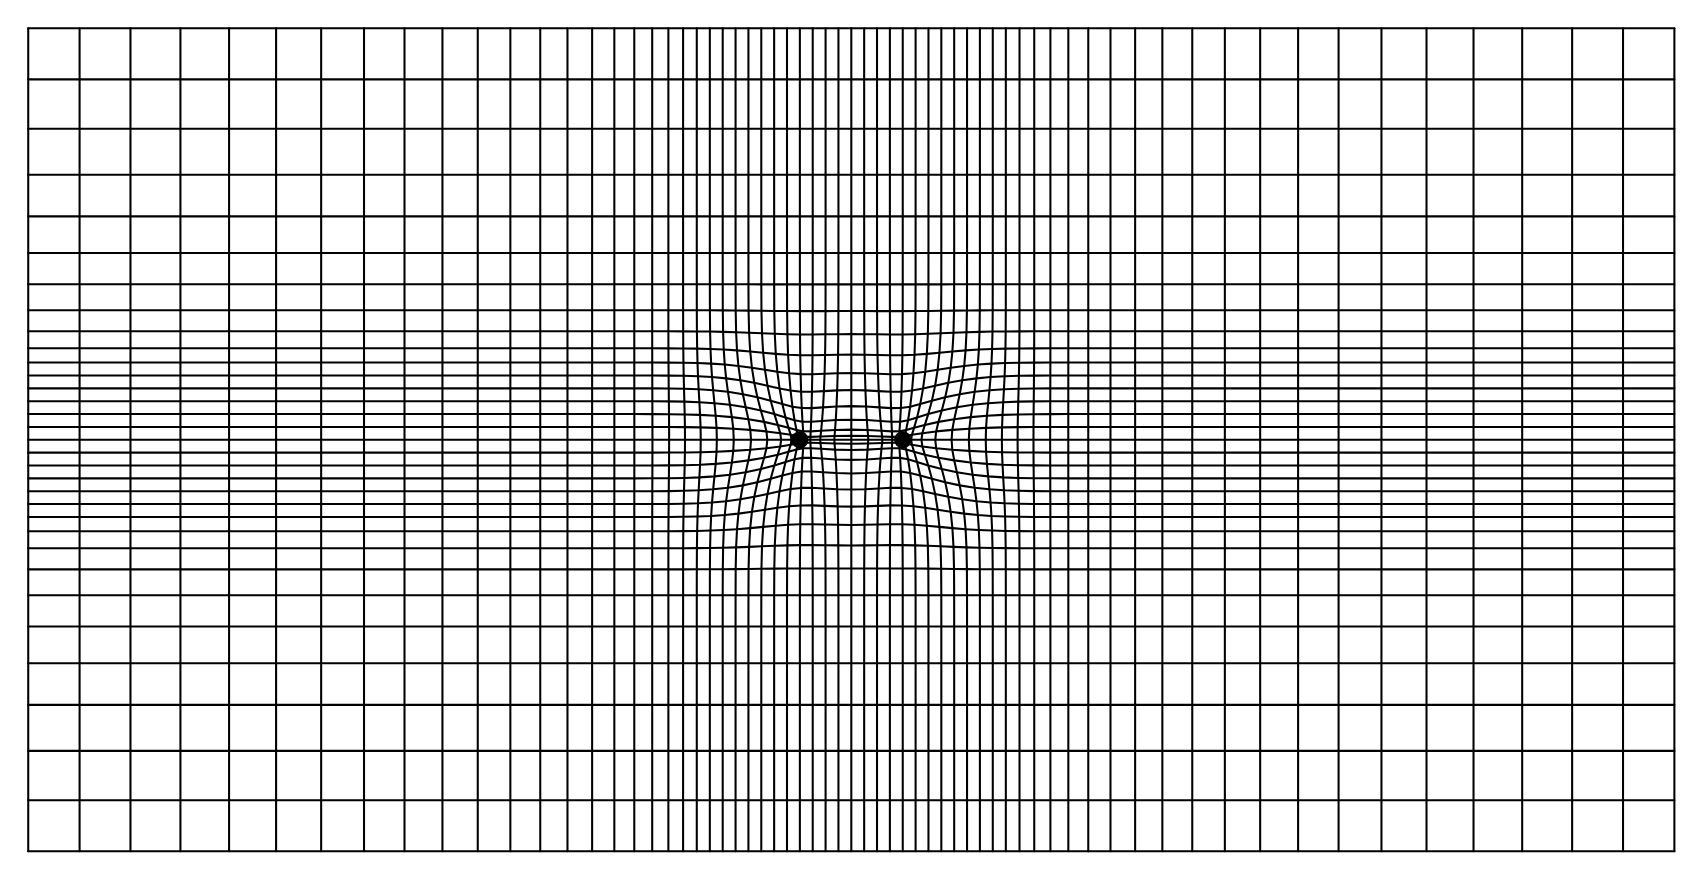
\includegraphics[width=.4\linewidth]{fig/adpative_grid.jpg}
		\end{figure}
		\item Solve some OT-type problems to predetermine the grid before the SCF
		loop: Lindsey and Sharma (2024)
	\end{itemize}
	
	Thought: the design of the distorted grid has great freedom and has to be done by expert 
	for each crystal system -- can we have a more adaptive and automatic design
	of the distorted grid?
\end{frame}


\begin{frame}{Normalizing flow on periodic domain}

	\begin{itemize}
		\item Invertible mapping on $S^1$ parametrized by spline function, Durkan et al. (2019)
		\begin{figure}[h]
			\centering
			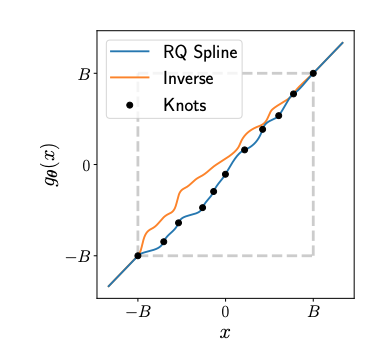
\includegraphics[width=.4\linewidth]{fig/nsf.jpg}
			% \caption{Figure from Durkan et al. (2019)}
		\end{figure}
		\item Coupling layer to handle 3D domain:
		\begin{equation*}\label{equ:cnf-auto-regressive}
			\begin{pmatrix}
			x_1^{(0)} \\
			x_2^{(0)}
			\end{pmatrix} 
			\underset{x_2^{(1)}=\ x_2^{(0)}}{\xrightarrow{x_1^{(1)}=\ \phi(x_1^{(0)}, \text{NN}^{(1)}_2(x_2^{(0)}))}}
			\begin{pmatrix}
			x_1^{(1)} \\
			x_2^{(1)}
			\end{pmatrix} 
			\underset{x_2^{(2)}=\ \phi(x_2^{(1)},\, \text{NN}^{(1)}_2(x_1^{(1)}))}{\xrightarrow{\quad\quad x_1^{(2)} =\ x_1^{(1)} \quad\quad }}
			\begin{pmatrix}
			x_1^{(2)} \\
			x_2^{(2)}
			\end{pmatrix}
		\end{equation*}
		\item Autoregressive layer to improve expressivity
	\end{itemize}
\end{frame}


\begin{frame}{Distorted plane-wave basis}
	\begin{itemize}
		\item Given invertible mapping $f: \Omega \to \Omega$, define distorted planewaves (DPW) $\phi _{\vb{G}}$ as planewaves in the parameter space:
		\begin{equation*} \label{eqn:dpw}
		\braket{\vb{r}}{\vb{G}} := \phi _{\vb{G}}(\vb{r})
			= \frac{1}{\sqrt{|\Omega|}} \abs{ J_{f^{-1}}(\vb{r})}^{\frac{1}{2}} \exp \left[\I \vb{G} ^{\top} f^{-1}(\vb{r})  \right]
		\end{equation*}
		\item Bloch factor
		\item Kinetic energy; Hartree energy; XC energy; Ewald summation
	\end{itemize}
\end{frame}


\begin{frame}{Kinetic matrix element: FFT}
	\begin{itemize}
		\item Matrix element involves Jacobian of the mapping:
		\begin{equation*}
			\begin{split}
		& \mel{\psi _{i, \vb{k}}}{-\frac{1}{2}\nabla^2}{\psi _{j, \vb{k}}} \\
				=& \frac{1}{2} \sum_{\vb{G}', \vb{G}} c^{*}_{i, \vb{k}, \vb{G}'} 
				c_{j, \vb{k}, \vb{G}}\{B_{\vb{G}', \vb{G}} - G_{q}[U_{\vb{G}', \vb{G}}]_{q} 
				+ G'_{q}[U_{\vb{G}', \vb{G}}]_{q} + (G_{p}+k_{p})(G'_{q}+k_{q})[P_{\vb{G}', \vb{G}}]_{pq}\}
			\end{split}
		\end{equation*}
		\item $B, U, P$ are all block-Toeplitz
		\item FFT implementation of the Toeplitz matrix-vector product is extremely fast
	\end{itemize}
\end{frame}


\begin{frame}{Hartree energy: solving the Poisson equation}
	\begin{equation*}
		\laplacian V = -4\pi \rho
	\end{equation*}
	\begin{itemize}
		\item Solved by FFT in plane-wave basis
		\item Solved by physics-informed neural network (PINN) -- introducing an inner
		loop of optimization
		\item The loop of PINN needs not to be converged for each step, amortizing with
		the outer loop
	\end{itemize}
	\textbf{\color{red} Similar philosophy as the previous adaptive Gaussian
	basis.}
\end{frame}


\begin{frame}{Overall algorithm}
	\begin{itemize}
		\item \textbf{Input:} Crystal system parameters, init params of NF, PINN, coefficient
		\item \textbf{While} $E_{\text{total}}$ not converged:
		\begin{itemize}
			\item Calculate the Jacobian of the NF at each grid point
			\item Calculate the kinetic and XC energy
			\item \textbf{For} $i = 1, 2, \ldots, N_{\text{PINN}}$:
			\begin{itemize}
				\item Sample the collocation points $\{\mathbf{r}_i\}$ for PINN evaluation
				\item Calculate the PINN loss: $\frac{1}{N}\sum_{i=1}^N (\nabla^2 V_{\theta}(\mathbf{r}_i)
				+ 4\pi \rho(\mathbf{r}_i))^2$
				\item Backpropogate to update the PINN parameters
			\end{itemize}
			\item Calculate the Hartree energy 
			\item Backpropogate through the total energy
		\end{itemize}
		\item \textbf{Output:} Total energy $E_{\text{tot}}$, params of NF, PINN, coefficient
	\end{itemize}
\end{frame}


\begin{frame}{Good features}
	\begin{itemize}
		\item The orthonormality of the basis is preserved
		\item Calculation of the density related energy can be estimated 
		efficiently by the Monte-Carlo method instead of integrating over the
		grid:
		\begin{equation*}
			E_{\text{xc}} = \int_{\Omega} \epsilon_{\text{xc}}^{\text{LDA}}(\rho(\mathbf{r}))
			\rho(\mathbf{r})d\mathbf{r} = \frac{1}{N} \sum_{i=1}^N \epsilon_{\text{xc}}^{\text{LDA}}(\rho_i)
		\end{equation*}
		\item Comparing to results like, our method generates the grid on the fly and
		adatively during the optimization loop
		\item It can reduce the total grid size by $8$ times on small crystal systems
	\end{itemize}
\end{frame}


\begin{frame}{Numerical results}
	\begin{table}[htbp]
		\footnotesize
	\centering
	\caption{Band structure calculation for diamond with LDA. All energies are in eV unit.}
	{\tabulinesep=1.2mm
	\begin{tabu}{cccccc}
	\hline
	Method & FFT grid size & band gap & L & X & $\Gamma$  \\ \hline\hline
	\multirow{3}{*}{PW}
	 & 128 & 3.05869 & 7.51526 & 3.05869 & 4.79634  \\ \cline{2-6}
	 & 96  & 3.14795 & 7.61833 & 3.14795 & 4.77946  \\ \cline{2-6}
	 & 64  & 3.68519 & 7.72595 & 3.68519 & 4.88759  \\ \cline{2-6}
	\hline\hline
	\multirow{3}{*}{PW + ANC}
	 & 96 & 3.08192 & 7.7782  & 3.08192 & 4.75455  \\ \cline{2-6}
	 & 64 & 3.10424 & 7.77621 & 3.10424 & 4.88761  \\ \cline{2-6}
	 & 48 & 1.98104 & 7.39363 & 1.98104 & 4.84532  \\ \cline{2-6}
	\hline\hline
	\multirow{1}{*}{FDPW + PINN}
	 & 48 & 3.01882 & 7.26194 & 3.01882 & 4.41584  \\ \cline{2-6}
	\hline
	\end{tabu}}
	\end{table}
\end{frame}


\section{Machine-Learning Exchange-Correlation functional under Projector Augmented-Wave method}
\begin{frame}
	\centering
	\Large
	\textcolor{blue}{\insertsection}\\
	\vspace{1cm}
	\normalsize
	\begin{itemize}
		\item Implement PAW differentiably in \textit{Jrystal} package
		\item Implement MLXC under PAW formulation
	\end{itemize}
\end{frame}


\begin{frame}{PAW: domain decomposition}
	Motivation:
	\begin{itemize}
		\item Near atomic sites, influence of other atoms is negligible -- 
		atomic configuration
		\item At the interatomic region, the wavefunction is smooth and plane-wave
		is efficient
		\item Need a clever way to glue together above two parts of the wavefunctions
	\end{itemize}

	Procedure:
	\begin{itemize}
		\item Generate the pseudopotential from atomic DFT calculation, need to specify
		the XC functional
	\end{itemize}
\end{frame}


\begin{frame}{Diagrammtic illustration of PAW}
	\textbf{PAW is not a pseudopotential method! --- Bl\"{o}chl}
	\begin{figure}[h]
		\centering
		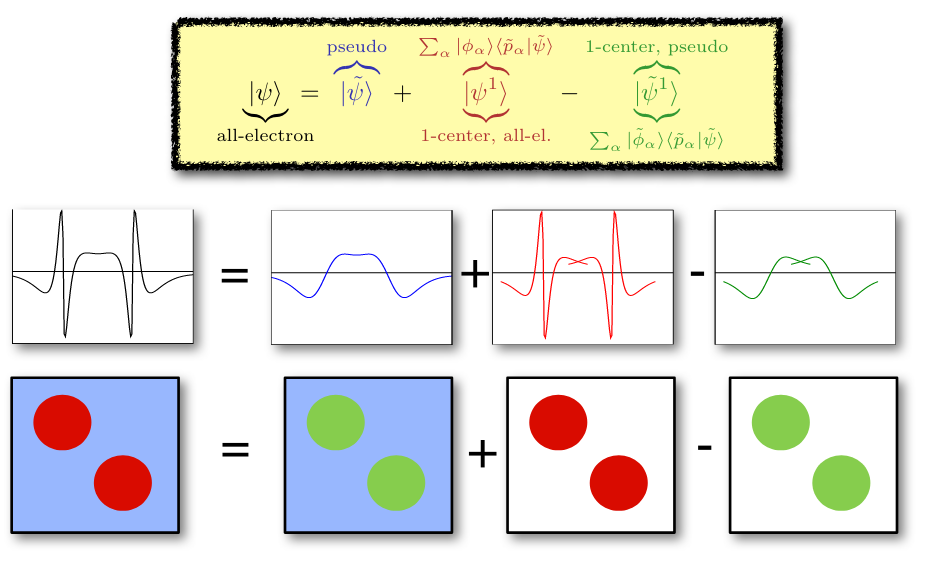
\includegraphics[width=.8\linewidth]{fig/paw_bloch.jpg}
		\caption{From Bl\"{o}chl's slide}
	\end{figure}
\end{frame}


\begin{frame}{Diagrammtic illustration of PAW}

	\begin{equation*}
			\begin{aligned}
				& \text{Wavefunctions:} \qquad \psi & = & \ \wtd \psi + \sum_a (\psi^a - \wtd\psi^a)		\\
				& \text{Density:} \qquad \qquad \rho & = & \ \wtd \rho + \sum_a (\rho^a - \wtd \rho^a)		\\
				& \text{Energy:} \qquad \qquad E_{\text{kin}} & = & \ \wtd E_{\text{kin}} +
				\half\sum_{a,i,j}D_{ij}^a
				\int_{\mathbb{S}^a}\lp \nabla{\phi_i^{a}}^*(\mathbf{r}) \nabla\phi_j^a(\mathbf{r}) - 
				\nabla\wtd {\phi_i^{a}}^*(\mathbf{r}) \nabla\wtd\phi_j^a(\mathbf{r}) \rp d\mathbf{r}		\\
			\end{aligned}
	\end{equation*}
	\begin{itemize}
		\item PAW is an all-electron theory with rigorous mathematical formulation
		and controllable errors.
		\item The pseudopotential generating process and PAW calculation process are
		``decoupled''.
	\end{itemize}
\end{frame}


\begin{frame}{Alignment platform with GPAW}
	\begin{itemize}
		\item Understand the mathematical derivation of the PAW
		\item Handle the difference of the pseudopotential file systems used by
		ours and GPAW
		\item Design of the unit test in the code development of the PAW
		\item First attempt to implement the MLXC under the PAW framework
	\end{itemize}
\end{frame}


\begin{frame}{MLXC for molecules v.s. materials}
	\begin{itemize}
		\item Golden standard computational method for molecules, CCDS(T) v.s. QMC for materials?
		\item Various datasets for molecules: QM9, etc v.s. MP for materials
		\item Pseudopotential is always included in the planewave calculations for material
		\item MLXC on molecules systems: DeepKS (Chen et al. 2020), DM21 (Kirkpatrick et al. 2021),
		Skala (Luise et al. 2025) 
	\end{itemize}
\end{frame}


\begin{frame}{The drawback of MLXC under NCPP \& USPP}
	\begin{itemize}
		\item The total energy and Hamiltonian contains a nonlinear core
		correction due to nonlinearity of the exchange-correlation potential
		\begin{equation*}
			V_{\text{xc}} = V_{\text{xc}}[\wtd \rho] + \sum_a (V_{\text{xc}}
			[\wtd \rho + \rho^{\text{core}}] - V_{\text{xc}}[\wtd \rho]).
		\end{equation*}
		\item The correction term is linearized, introducing error
		\item The XC potential is included in the local part of the pseudopotential
		and is unchanged even using different XC for calculation
	\end{itemize}
	
\end{frame}


\begin{frame}{Explicitly handle the XC energy}


	\begin{equation*}
		E_{\text{xc}} = E_{\text{xc}}[\wtd \rho] + \sum_a (E_{\text{xc}}^a[\rho] - E_{\text{xc}}^a[\wtd \rho])
	\end{equation*}
	\begin{itemize}
		\item $E_{\text{xc}}[\wtd \rho]$: the XC energy for the pseudo-density, integrated
		over uniform grid
		\item $E_{\text{xc}}[\rho^a] - E_{\text{xc}}[\wtd \rho^a]$: the XC energy difference of the
		on-site part
		\item The XC energy of the pseudopotential part is calculated by the MLXC functional
	\end{itemize}
\end{frame}


\begin{frame}{Design of loss function}
	\begin{itemize}
		\item High accuracy label for the crystal data is extremely sparse and expensive
		\item Training over the labels generated by the hybrid or double hybrid functional, e.g. HSE06
		\item Training over the set of stable material:
		\begin{equation*}
			\min \text{Tr}(\nabla_{\mathbf{r}} E(\mathbf{r}))
		\end{equation*}
	\end{itemize}
	
\end{frame}


\begin{frame}{An abstraction of SciML workflow}
	Simulating the dynamics:
	\bequn
		\begin{aligned}
			\mcL(\mfu, \p_t \mfu, \mfy, t) & = \mathbf{0}, 		\\
			\mfy & = \phi(\mfu, t).
		\end{aligned}
	\eequn
	\begin{itemize}
		\item 1. $\mcL$ is known, possibly non-linear, {\color{red}while $\phi$ is un-known}
		\item 2. Datasets: $\lbb (\mfu_1, \mfy_1, t_1), (\mfu_2, \mfy_2, t_2), \cdots, (\mfu_N, \mfy_N, t_N )\rbb$
		\item 3. {\color{red} Benchmark algorithm solves the ordinary least square:
		\bequn
			\arg\min_{\theta} \mbE \norml \mfy - \phi_{\theta}(\mfu, t) \normr^2
		\eequn}
	\end{itemize}
	
	Typical examples: subgrid-scale modeling, reynolds stress modeling, exchange-correlation functional

\end{frame}


\begin{frame}{A-priori and a-posteriori discrepancy}
	\begin{itemize}
		\item Models performing well a-priorily may not perform well in the simulation
		\item Training algorithm does not take the solver dynamics into account
	\end{itemize}
	\begin{figure}
		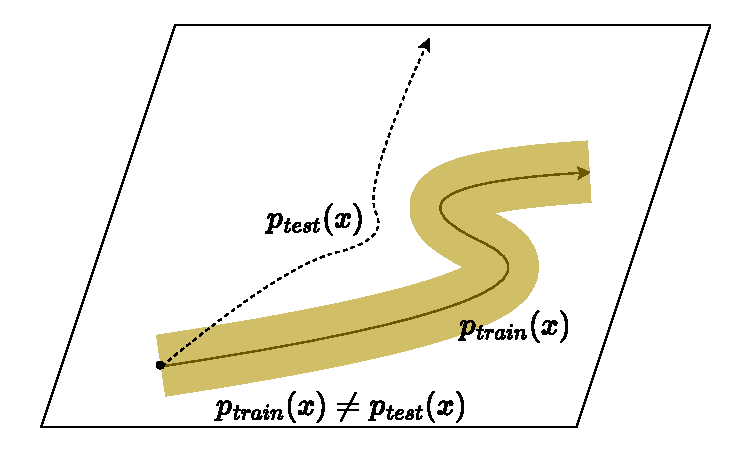
\includegraphics[width=.6\textwidth]{fig/ds.pdf}
		\label{fig:dilemma}
	\end{figure}
\end{frame}


\begin{frame}{Alg 1: Manifold regularization\footnotemark[1]}
	\begin{itemize}
		\item Regularization encodes the information of the data manifold
		\item Assume $u_2 \in \alpha, u_1 \in \alpha, \left\| u_0 - u_1 \right\| = \left\| u_0 - u_2 \right\|$
		\begin{figure}[H]
			\centering
			\centerline{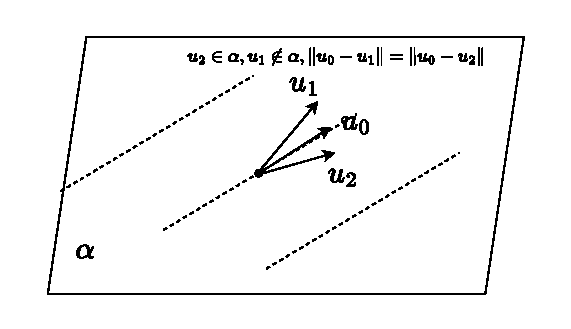
\includegraphics[width=0.6\linewidth]{fig/tr.pdf}}
		\end{figure}
		\begin{equation*}
			l_{\text{TR}}(\theta) := \mbE_{(\mfu, \mfy)}\lb \norml \mfy_k - \phi_{\theta}(\mfu) \normr_2^2
			+ \lambda \lp\lp  \nabla F(\mfu) \rp^T L(\mfu, \phi_{\theta}(\mfu), t)\rp^2 \rb
			\end{equation*}
	\end{itemize}
	\footnotetext[1]{Zhao, Jiaxi, and Qianxiao Li. "Mitigating Distribution Shift
	in Machine Learning–Augmented Hybrid Simulation." SIAM Journal on
	Scientific Computing 47.2 (2025): C475-C500.}
\end{frame}


\begin{frame}{Alg 2: Probabilistic ansatz\footnotemark[2]}
	Regression to generative modeling:
	\begin{equation*}
    \tau = \phi_{\theta}(\mfu) \quad \rightarrow \quad \tau \sim p_{\theta}(\cdot|\mfu)
	\end{equation*}

	Change of the loss functions:
	\begin{equation*}
   \min_{\theta} \sum_{n} \norml \phi_{\theta}(\wtd{\mfu}^{(n)}) - \tau^{(n)} \normr^2,\quad
	 \max_{\theta}\sum_{i=n}^{N}\log p_{\theta}(\tau^{(n)}|\mfu^{(n)})
	\end{equation*}
	\footnotetext[2]{Zhao, Jiaxi, Sohei Arisaka, and Qianxiao Li. 
	"Generative subgrid-scale modeling." ICLR 2025 Workshop on Machine
	Learning Multiscale Processes}
\end{frame}


\begin{frame}{Alg 3: Correction-based SGS models}
	Considering a PDE with both linear and nonlinear terms
	\begin{equation*}
		\partial_t \overline{u} + \mathcal{L}(\overline{u}) + \mathcal{N}(\overline{u}) + \tau(\overline{u}) = 0
	\end{equation}
	\begin{itemize}
		\item Filter-based approach:
		\begin{equation*}
			\mathcal{F}(u^f) = u^c \Longrightarrow \tau^{(1)} = 
			\mathcal{F}(\mathcal{N}(u^f)) - \mathcal{N}(u^c)
	\end{equation*}
		\item Correction-based approach:
		\begin{equation}
			\mathcal{F}(u^f) = u^c \Longrightarrow \tau^{(2)} =
			\mathcal{F}(\text{solver}^f(u^f)) - \text{solver}^c(u^c)
	\end{equation}
	\end{itemize}
	
\end{frame}


\begin{frame}
	Thank you for your attention!
	Q \& A
	\begin{itemize}
		\item Email: \href{mailto:jiaxi.zhao@u.nus.edu}{jiaxi.zhao@u.nus.edu} 
		\item WeChat:
		\begin{figure}[ht] 
			\centering 
			
\includegraphics[width=.3\textwidth]{fig/qrcode.jpg} 
		\end{figure}
	\end{itemize}
\end{frame}


% \begin{frame}{Potential improvement}
% 	\begin{itemize}
% 		\item Using greedy algorithm to optimize for more Gaussian modes, i.e.
% 		one can use the optimization results for less modes as the warm-start
% 		for more modes
% 		\item The approximation interval $[0, M]$ can be done adaptively according
% 		to the relative position of two Gaussian modes
% 		\item Motivated by the Boys function, can we design other decomposition
% 		of the Coulomb kernel?
% 		\begin{equation*}
% 			\frac{1}{r} = C\int_{\mbR} e^{-r^2t^2} dt
% 		\end{equation*}
% 	\end{itemize}
% \end{frame}


% \begin{frame} % Use [allowframebreaks] to allow automatic splitting across slides if the content is too long
%     \frametitle{References}
 
%     \begin{thebibliography}{99} % Beamer does not support BibTeX so references must be inserted manually as below, you may need to use multiple columns and/or reduce the font size further if you have many references
%         \footnotesize % Reduce the font size in the bibliography
 
% 		\bibitem[migbs]{migbs}
% 		Gill, Peter MW.
% 		\newblock Molecular integrals over gaussian basis functions.
% 		\newblock \emph{Advances in quantum chemistry. Vol. 25. Academic Press,
% 		1994. 141-205.}

% 		\bibitem[3dgs]{3dgs}
% 		Kerbl, Bernhard, et al
% 		\newblock 3D Gaussian Splatting for Real-Time Radiance Field Rendering
% 		\newblock \emph{ACM Trans. Graph. 42.4 (2023): 139-1.}

% 		\bibitem[S.A. and Q.L., 2024]{nigbms}
% 		S. Arisaka and Q. Li (2024)
% 		\newblock Accelerating Legacy Numerical Solvers by Non-intrusive Gradient-based Meta-solving
% 		\newblock \emph{International Conference on Machine Learning 2024}
 
        
%     \end{thebibliography}
% \end{frame}

\end{document}